\documentclass[12pt]{article}
\usepackage[utf8]{inputenc}
\usepackage{graphicx}
\graphicspath{ {images/} }
\usepackage{multicol}
\setlength{\columnsep}{2cm}


\usepackage[cp1251]{inputenc}
\usepackage[russian]{babel}



\begin{document}

\begin{titlepage}
	\centering
	{\scshape\LARGE Московский физико-технический институт \par}
	\vspace{3cm}
	{\scshape\Large Лабораторная работа по курсу\\ Вакуумная электроника \par}
	\vspace{1cm}
	{\huge\bfseries Электроконтактная сварка \par}
	\vspace{1cm}
	\vfill
\begin{flushright}
	{\large выполнила студентка 653 группы ФФКЭ}\par
	\vspace{0.3cm}
	{\LARGE Карпова Татьяна} 
\end{flushright}

	\vfill

% Bottom of the page
Долгопрудный, 2017 г.
\end{titlepage}

\newpage


\section{Цель работы}
\begin{enumerate}
    \item Изучить физические принципы электроконтактной сварки
    \item Овладеть основными приёмами различных сварочных операций
\end{enumerate}

\section{Виды электроконтактной сварки}
{\it Электроконтактная сварка} - комплексный электромеханический процесс, при котором нагрев места соединения производится проходящим через него электрическим током и сопровождается приложением усилий сжатия. \par 
Виды электроконтактной сварки:
\begin{itemize}
    \item {\it Точечная сварка} выполняется в виде отдельных точек с интервалом между ними. Одна из разновидностей точечной сварки - рельефная сварка.
    \item {\it Роликовая сварка} - при её выполнении соединение деталей производится с помощью вращающихся электродов-роликов. Роликовая сварка подразделяется на непрерывную (непрерывная подака тока в сварочную цепь и образование ряда точек, перекрывающих друг друга, в результате чего получается сплошной герметичный шов), и прерывистой (на ролики подаются кратковременные импульсы тока, соединения не отличаются от выполненных точечно)
    \item {\it Стыковая сварка} - электрический ток проходит через стык соединённых деталей, разогревая их концы, после чего прилагается усилие сжатия.
\end{itemize}

\begin{figure}[h]
    \centering
    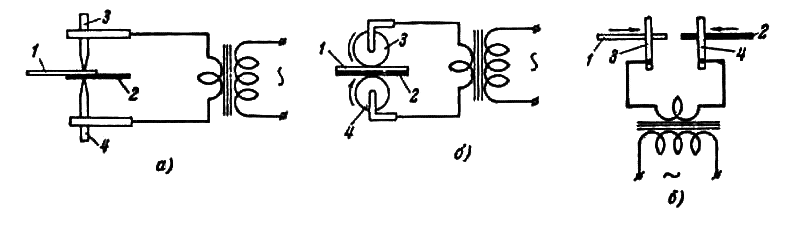
\includegraphics[width=7.5 cm]{weld_types.png}
    \caption{Виды электроконтактной сварки: а) — точечная, б) — роликовая, в) — стыковая; 1, 2 — свариваемые детали; 3, 4 – электроды}
    \label{fig:vac}
\end{figure}

\section{Требования к сварочным соединениям}

При изготовлении электровакуумных приборов часто необходимо изготовление неразъёмных соединений деталей, выполненных из металлов с различными электрофизическими свойствами. Более 90\% всех сварных соединений в электровакуумной технике производится с помощью электроконтактной сварки.\par
Требования к таким соединениям:
\begin{enumerate}
    \item Высокая статическая и динамиеская прочность при длительной работе в вакууме и при других нагрузках
    \item Высокая электро- и теплопроводность
    \item Соответствие требованиям вакуумной чистоты (отсутствие шлаков, летучих соединений, других посторонних частиц)
\end{enumerate}

Качество соединений зависит от:
\begin{itemize}
    \item Предварительной подготовки поверхности деталей (полировка, обезжиривание)
    \item Усилия сжатия
    \item Сварочного тока
    \item Времени сварки.
\end{itemize}

\section{Принципы работы сварочного оборудования}
По способу получения сварочного тока электроконтактная сварка разделяется на трансформаторную и импульсную. \par
{\it Трансформаторная сварка} используется в случаях, когда приходится производить сварку в сильно различающихся режимах и высокая производительность не важна. Усилие сжатия и время прохождения тока определяются сварщиком, поэтому качество сварки напрямую зависит от его квалификации. Трансформаторная сварка не позволяет работать в режиме, требующем короткого времени сварки. \par 
{\it Импульсная сварка} используется для режимов, требующих короткого времени сварки. Формирование импульса напряжения проиходит только после достижения требуемого механического усилия на детали. Импульсные формирователи обычно выполняют по {\it тиристорной} или {\it конденсаторной} схемам. Детали во время сварки могут удерживаться как вручную, так и при помощи специальных оправок. Для повышения производительности и повторяемости сварочного процесса могут быть использованы автоматические установки с возможностью задания на них усилия сжатия, длительности и мощности сварочного импульса.  

\section{Лабораторная установка}

Лабораторная установка предстваляет собой пост импульсной электроконтактной сварки, снабжённый неподвижным нижним и ручным верхним электродами. Длительность сварочного импульса устанавливается оператором. \par 
Параметры сварки на установке:
\begin{itemize}
    \item {\it Длительность сварочного импульса} устанавливается в зависимости от того количества тепла, которое необхадимо выделить для образования ядра. Увеличение длительности импульса может привести к выплеску вследствие перегрева металла в ядре. При недостаточной длительности импульса ядро может не образоваться.
    \item {\it Величина усилия сжатия} устанавливается, учитывая прочность металлов и их термическую обработку. Эта величина должна оставаться постоянной в процессе сварки для получения одинаковых по качеству сварных точек. Снятие давление должно производиться через некоторое время после выключения сварочного тока, иначе в ядре могут возникнуть раковины и поры, препятствующие его уплотнению.
\end{itemize}

\section{Дефекты сварки}
Вследствие неправльного выбора режима сварки, неисправности оборудования или ошибок оператора могут возникунть различные дефекты при сварке.
\begin{enumerate}
    \item {\it Выплеск} расплавленного металла может образоваться в результате слишком большой длительности сварочного импульса, слишком малого давления на деталь, перекосом деталей, их загрязнением и другими факторами. Выплеск может стать причиной коротких замыканий. Наиболее часто происходит выплеск при соединени проволоки с проволокой или ленты с проволокой, так как плотность тока в этих случаях является наиолее высокой.
    \item {\it Непровар} - недостаточно прочное соединение свариваемых деталей. Его причиной могут стато неправильное расположение пинцета для захвата деталей, недостаточные длительность сварочного импульса и давление на деталь, а также загрязнение деталей
    \item {\it Прожог} - явление, при котором сварочная точка имеет глубокую вмятину  и форму, отличающуюся от формы электрода. Причиной прожога могут служить завышенные длительность сварочного импульса и сжатие электродов, а также перекос деталей при сварке и неправльная установка электродов.
\end{enumerate}

\newpage

\section{Практическая часть}

\begin{enumerate}
    \item Перед началом работы проведём пробную сварку на предложенных образцах, регулируя длительность сварочного импульса и усилие сжатия. Перед сваркой зачищаем свариваемые поверхности спиртом, пожвижный электрод зачищаем от остатков металла наждачной бумагой.
    \item Проведём подготовку деталей. Для изготовления анода нам потребуется лист никеля размером 30х40 мм. Избавляемся от неровностей на никелевой заготовке, прокатывая её между наковальней и рабочей пластиной. 
    \item На никелевой заготовке для придания аноду дополнительной жёсткости проведём рёбра жёсткости вдоль более длинной стороны. Готовый вид заготовки анода представлен на рисунке 3.
    \item Обернём никелевую заготовку вокруг оправкки с нахлёстом 3 мм, завальцуем края платины в шве. Необходимо, чтобы края плотно прилегали к поверхности оправки, иначе может образоваться зазор, приводящий к дефектам свариваемых точек.
    \item Произведём точечную сварку вдоль короткой стороны посередине нахлёста. Сначала сделаем две точки по краям нахлёста, затем одну посередине (это делается во изежание деформации сваочного шва), затем слева направо начнём производить сварку по всей длине нахлёста, выдерживая расстояние можде сварочными точками 2-3 мм. После каждой точни проворачиваем анод на оправке, так как он может привариться к ней.
    \item Изготовим траверсы дя крепления анода на точку. Для этого подготовим два отрезка никелевой проволоки длиной 50 мм, выпрямим их путём проката между пластинами наковальни. 
    \item Приварим траверсы к аноду. Они должны располагаться диаметрально противоположно, но не располагаться на шве. Сварка производится точечно, действия аналогичные пункту 5. Вид заготовки с приваренными траверсами предствлен на рисунке 4.
    \item В ходе приварки траверса к аноду произошёл выплеск, вследствие чего повредилась проволока и необходимо было изготовить заплатку. Для изготовления заплатки возьмём небольшой отрезок проволоки и приварим его к траверсу с двух сторон от повреждённого участка.
    \item Изготовим натягивающую траверсу: возьмём отрезок никелевой проволоки длиной 80 мм, выпрямим его, прокатав на наковальне. Возьмём лист никеля размером 3х8 мм, согнём его пополам и соединим с натягивающей траверсой. Траверсу изогнём под прямым углом. 
\end{enumerate}

\begin{figure}[h]
\begin{multicols}{2}
\hfill
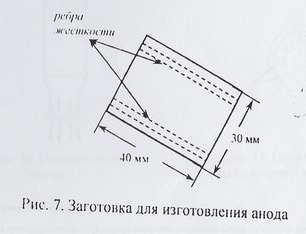
\includegraphics[width=60mm]{anode.png}
\hfill
\caption{Заготовка анода}
\label{figLeft}
\hfill
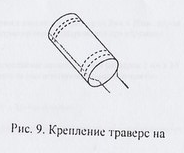
\includegraphics[width=50mm]{trav.png}
\hfill
\caption{Схема приварки траверс}
\label{figRight}
\end{multicols}
\end{figure}

\section{Вывод}
В ходе работы мы ознакомились с принципами работы сварочного оборудования, используемого в электровакуумном производстве, его основными характеристиками. Были изучены различные дефекты, возникающие при сварке, и причины их возникновения. При выполнении практической части были проведены простейшие сварочные операции (сварка пластина-пластина, пластина-проволока), изготовлены заготовка анода и траверсы.

\end{document}
